% Copyright 2019 Clara Eleonore Pavillet

% Author: Clara Eleonore Pavillet (original author), Leonard Quentin Marcq (modified for Tsinghua), 赵宗义 (参与了修改)
% Description: This is an unofficial Tsinghua University Beamer Template I made from scratch. Feel free to use it, modify it, share it.
% Version: 1.1

\PassOptionsToPackage{quiet}{xeCJK}
\documentclass{beamer}
\usepackage{ctex}
\usepackage{fontspec}
% Load Packages
% \usepackage[utf8]{inputenc}
\usepackage{xcolor}
\usepackage{tikz}
\usetikzlibrary{positioning,calc}
\usepackage{graphicx}
\usepackage{hyperref}
\usepackage{amsmath}
\usepackage{listings}
%\usepackage{fontawesome}

% Define Commands
\newcommand*{\ClipSep}{0.06cm} %To adjust footer logo
\newcommand{\E}{\mathrm{e}\,} %\def\I{e} % used to defined e for exp(x), see later what it should be
\newcommand{\ud}{\mathrm{d}}
\lstset{numbers=left, numberstyle=\tiny, stepnumber=1,firstnumber=1,breaklines=true,
    numbersep=5pt,language=Python,
    stringstyle=\ttfamily,
    basicstyle=\footnotesize, 
    showstringspaces=false
}

\usetheme{iscastca}

%%%<<<---
\newcommand{\system}{Crystals-Kyber}
\newcommand{\variable}{\mathrm}
\newcommand{\field}{\mathsf}
%%%--->>>
\title{This is the title}
\subtitle{This is the subtitle}
\author{Author}
\institute{中国科学院软件研究所}
\date{\today} %\today

\begin{document}

{\setbeamertemplate{footline}{} 
\frame{\titlepage}}



\begin{frame}{{\system}的总体架构}
\textbf{困难问题}
\begin{enumerate}
\item Factoring
\item Discrete log
\end{enumerate}
\textbf{量子算法}
\begin{enumerate}
\item Shor's 算法
\item Grover 算法 (量子搜索算法)
\end{enumerate}
\end{frame}

\begin{frame}{数据平面}
\begin{enumerate}
\item 数据平面包含了两个哈希表, 分别是主表 (Main Table) 和辅表 (Ancillary Table).
\item 主表中每个哈希桶包含两个域: $\field{fieldID}$和$\field{count}$
\item 辅表中每个哈希桶也包含两个域: $\field{digest}$和$\field{count}$
\end{enumerate}
\begin{figure}
	\centering
	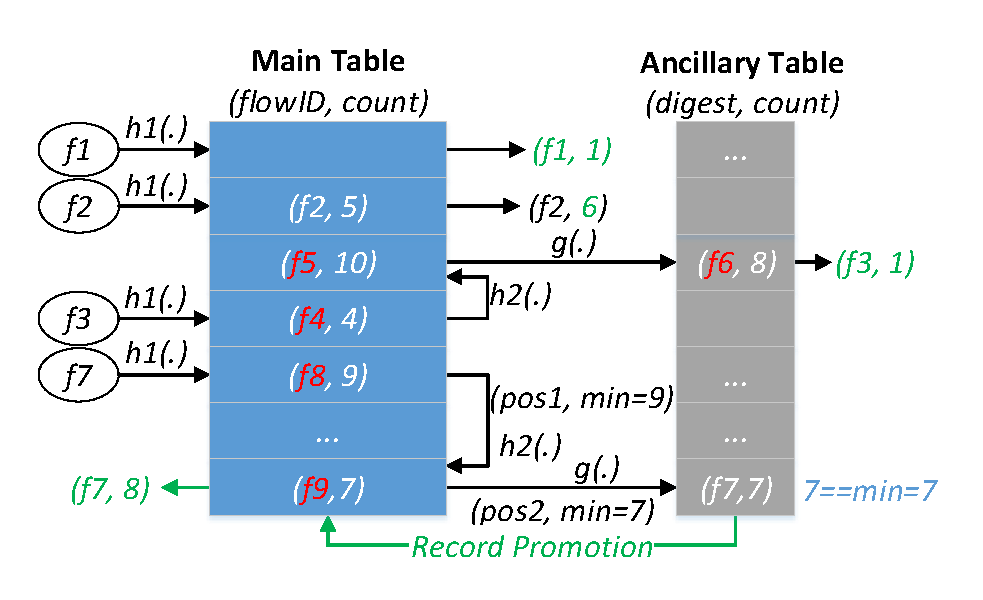
\includegraphics[width=0.6\linewidth]{figures/representation/datastructure}
\end{figure}

\end{frame}

\usebeamertemplate{endpage}

\end{document}

